\documentclass{beamer}
\usepackage[right]{eurosym}
\usepackage{latexsym}
\usepackage{pgf,pgfarrows,pgfnodes,pgfautomata,pgfheaps}
\usepackage{color}
\usepackage{bbm}
\usepackage[english]{babel}
\usepackage[utf8]{inputenc}
% \usepackage[vmargin=25mm, top=20mm, bottom=25mm, left=28mm, right=28mm, includehead]{geometry}
% \usepackage{parskip}
\usepackage{csquotes}
\usepackage{german}
\usepackage{ngerman}
\usepackage{microtype}
\usepackage{amsfonts}
\usepackage{amssymb}
\usepackage{amsmath}
\usepackage{graphicx}
\usepackage{extarrows}
\usepackage{amsthm}
\usepackage{bookmark}
\usepackage{mathrsfs}
\usepackage{scrextend}
\usepackage{tikz}
\usepackage{subcaption}
\usepackage{float}
\usepackage{mathtools}
\usepackage{wrapfig}
\usepackage[singlelinecheck=false,justification=justified]{caption}
\usepackage[ruled,vlined]{algorithm2e}
\usepackage{algpseudocode}
\usepackage{mathtools}
\usepackage{hyperref}
\usepackage{graphicx}
\usepackage{times}
\usepackage[T1]{fontenc}


\graphicspath{{./graphics/}}

\usepackage[
    left = \flqq{},%
    right = \frqq{},%
    leftsub = \flq{},%
    rightsub = \frq{} %
]{dirtytalk}


\bibliographystyle{acm}

\newcommand{\uz}{\wegde}
\newcommand{\oz}{\vee}
\newcommand*\xor{\mathbin{\oplus}}
\everymath{\displaystyle}
\newcommand{\N}{\mathbb{N}}
\newcommand{\Prob}{\mathbb{P}}
\newcommand{\Z}{\mathbb{Z}}
\newcommand{\R}{\mathbb{R}}
\newcommand{\Q}{\mathbb{Q}}
\newcommand{\C}{\mathbb{C}}
\newcommand{\source}[1]{\caption*{Source: {#1}} }
\captionsetup[figure]{font=footnotesize}
\usepackage{commath}
\usepackage{esdiff}
\DeclareMathOperator{\Var}{\mathbf{Var}}
\DeclareMathOperator{\EW}{\mathbf{E}}
\DeclareMathOperator{\WS}{\mathbf{P}}
\DeclareMathOperator{\Cov}{\mathbf{Cov}}
\newcommand{\notimplies}{\;\not\!\!\!\implies}
% Set up

\mode<presentatio>
{
  \usetheme{Warsaw}
  \setbeamercovered{transparent}
}
\setbeamersize{text margin right = 20mm, text margin right= 20mm}
% Oder was auch immer. Zu beachten ist, das Font und Encoding passen
% m�ssen. Falls T1 nicht funktioniert, kann man versuchen, die Zeile
% mit fontenc zu l�schen.

\title[]{TC-VAE: Uncovering Out of distribution generative factors}
\author{Andreas Loehr}
\institute{Goethe Universität Frankfurt a.M.}
\date{
  \vspace{0.2cm}
  Seminar Pattern Analysis and Machine Intelligence
  \vspace{0.4cm}
  \newline 06/22/2023\\
  \vspace{0.3cm} % 0.4cm
  }
\subject{Informatik}

\let\definition\relax
\let\theorem\relax
%\let\footnoterule\relax
% \let\theorem\relax
\theoremstyle{definition}
\newtheorem{definition}[section]{Definition}
\newtheorem{intuition}{Intuition}
% \newtheorem{definition_theorem}[definition]{Definition und Satz}

\newtheorem{cus_theorem}[section]{Satz}
%\newtheorem{def_theorem}[section]{Definition und Satz}
% \newtheorem{lemma}[definition]{Lemma}
% \newtheorem{remark}[definition]{Bemerkung}
% \newtheorem{remark_ex}[definition]{Beispiel}
% \newtheorem{notation}[definition]{Notation}
\newtheorem{remark}{Bemerkung}
\begin{document}
  \AtBeginSection[]
  {
      \begin{frame}
          \tableofcontents[currentsection]
      \end{frame}
    }
    % title page
  \begin{frame}
    \begin{titlepage}
    \end{titlepage}
  \end{frame}

  %intro to generative modelling. The problem statement
  \section{Representation Learning and Generative Modeling}
    \begin{frame}
      \frametitle{The Problem statement}
      \begin{itemize}
        \item \textbf{Problem}: Given data $X \in \mathbb{R}^{d}$ find a \textit{good} latent representation $Z \in \mathbb{R}^{m}$, $d, m \in \mathbb{N}$
        \item \textbf{Example}: $X$ images of colored 3D objects, $Z$ latent representation representing shape, texture, color etc.
      \end{itemize}
     \end{frame}

     \begin{frame}
      \frametitle{Example: 3D-shapes dataset}
      \begin{figure}
        \centering
        \includegraphics[scale=0.15]{3d_shapes.png}
        \captionsetup{justification=centering}
        \caption*{\tiny{Source: https://github.com/deepmind/3d-shapes/tree/master}}
      \end{figure}
      %\vspace{-0.8 cm}
      \begin{itemize}
        \item Generative Factors $=\{[floor, wall, object] color, scale, shape, orientation\}$
      \end{itemize}
     \end{frame}

      \begin{frame}
        \frametitle{Definitions and Notation (1)}
        \begin{itemize}
          \item \textbf{Data Generative Factors:} True underlying factors / attributes of the data or generation process
          \item \textbf{OOD Data Generative Factors:} Generative Factors without variability in dataset
          % explain: no variation of this factor in entire dataset, e.g. all objects are located in center of image for OOD factor camera perspective
          \item \textbf{Latent Representation:} A vector of latent variables
        \end{itemize}
      \end{frame}

      \begin{frame}
        \frametitle{Distentanglement}
        \begin{itemize}
          \item no precise definition for disentanglement
        \end{itemize}
        \begin{definition}[Bengion et al 2013]
          A latent respresentation is called \textit{disentangled} if for each latent variable, the change in 1 generative factor leads to a change in 1 latent variable.
        \end{definition}
      \end{frame}

    \begin{frame}
      \frametitle{What makes a good latent representation?}
      \begin{itemize}
        \item captures true generative factors of the dataset
        \item interpretable $\rightarrow$ Optimally, \enquote{bijection} between data generative factors $\leftrightarrow$ latent representation
        \item sufficiently informative (captures majority of data generative factors)
        \item balanced $\to$ no single factor outweighs other factor in terms of informativeness
        \item Regularity TODO
        \item TODO: completeness definition, condense the above
        %, i.e. generative factors underrepresented in training data still have correspoding latent factor factors underrepresented in training data still have correspoding latent factor factors underrepresented in training data still have correspoding latent factor
        % in the sense that even generative factors which are underrepresented in the dataset do have a correspoding latent factor
      \end{itemize}
    \end{frame}

    \begin{frame}
        \frametitle{Why bother to learn good representations?}
        \begin{itemize}
          \item Facilitate downstream tasks like classification
          \item Controllable Generative modeling: control generative factors explictly by tweaking the corresponding latent variables
          % TODO: add more reasons and illustrate
        \end{itemize}
      \end{frame}

    \section{(Variational) Autoencoders}
    \begin{frame}
      \frametitle{Means to learn latent representations}
      \begin{itemize}
        \item Principal component analysis (PCA)? $\rightarrow$ Lack of interpretability
        \item (Regular) Autoencoders? $\rightarrow$ Lack of regularity
        % explain regularity - refer to Medium article/ paper
        % https://towardsdatascience.com/understanding-variational-autoencoders-vaes-f70510919f73
        \item Variational Autoencoders (VAE) $\rightarrow$ Lack of disentanglement and/ or regularity
      \end{itemize}
    \end{frame}
    % Note: Now work towards the principal contribution of the paper

    \begin{frame}
      \frametitle{Autoencoders}
      % source autoencoder illustration
      %https://miro.medium.com/v2/resize:fit:4266/1*QEmCZtruuWwtEOUzew2D4A.png
      %\begin{center}
      \begin{figure}
        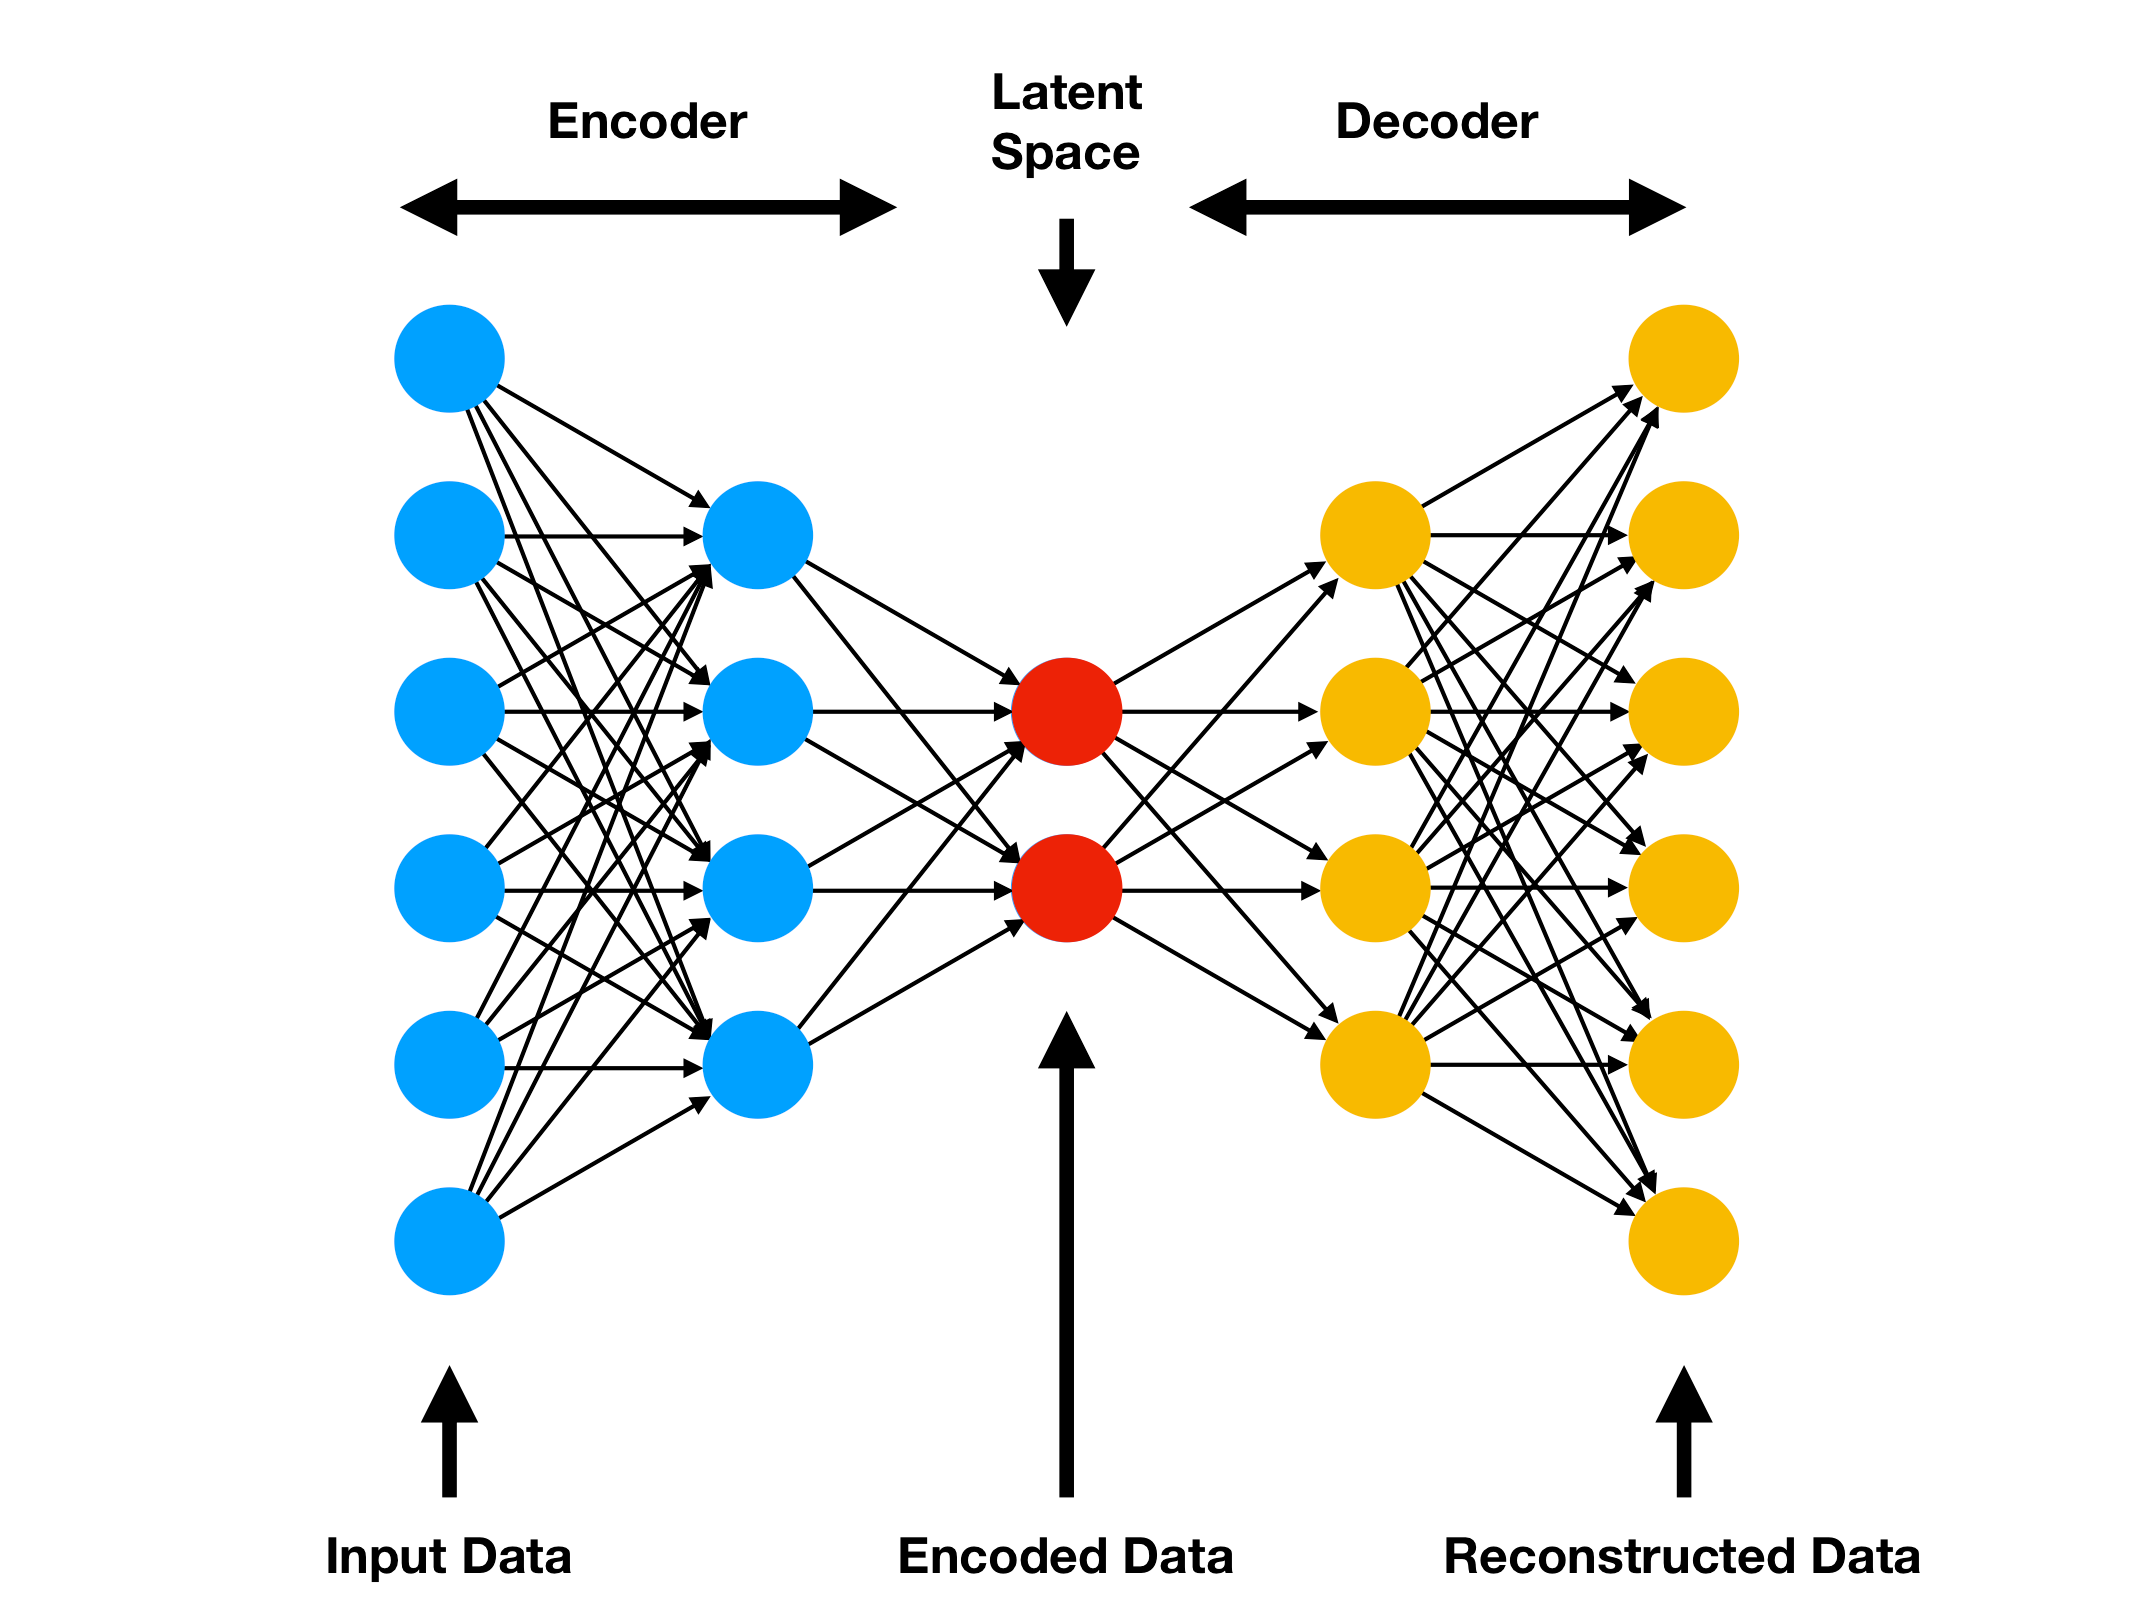
\includegraphics[scale= 0.09]{Autoencoder_illustration.png}
        \caption*{Source: https://medium.com/autoencoder-for-anomaly-detection/autoencoder-for-anomaly-detection-db6178ad07b2}
        % explain graphics quickly
      \end{figure}
      % \end{center}

    \end{frame}
    \begin{frame}
      \frametitle{Variational Autoencoders}
      \begin{figure}
        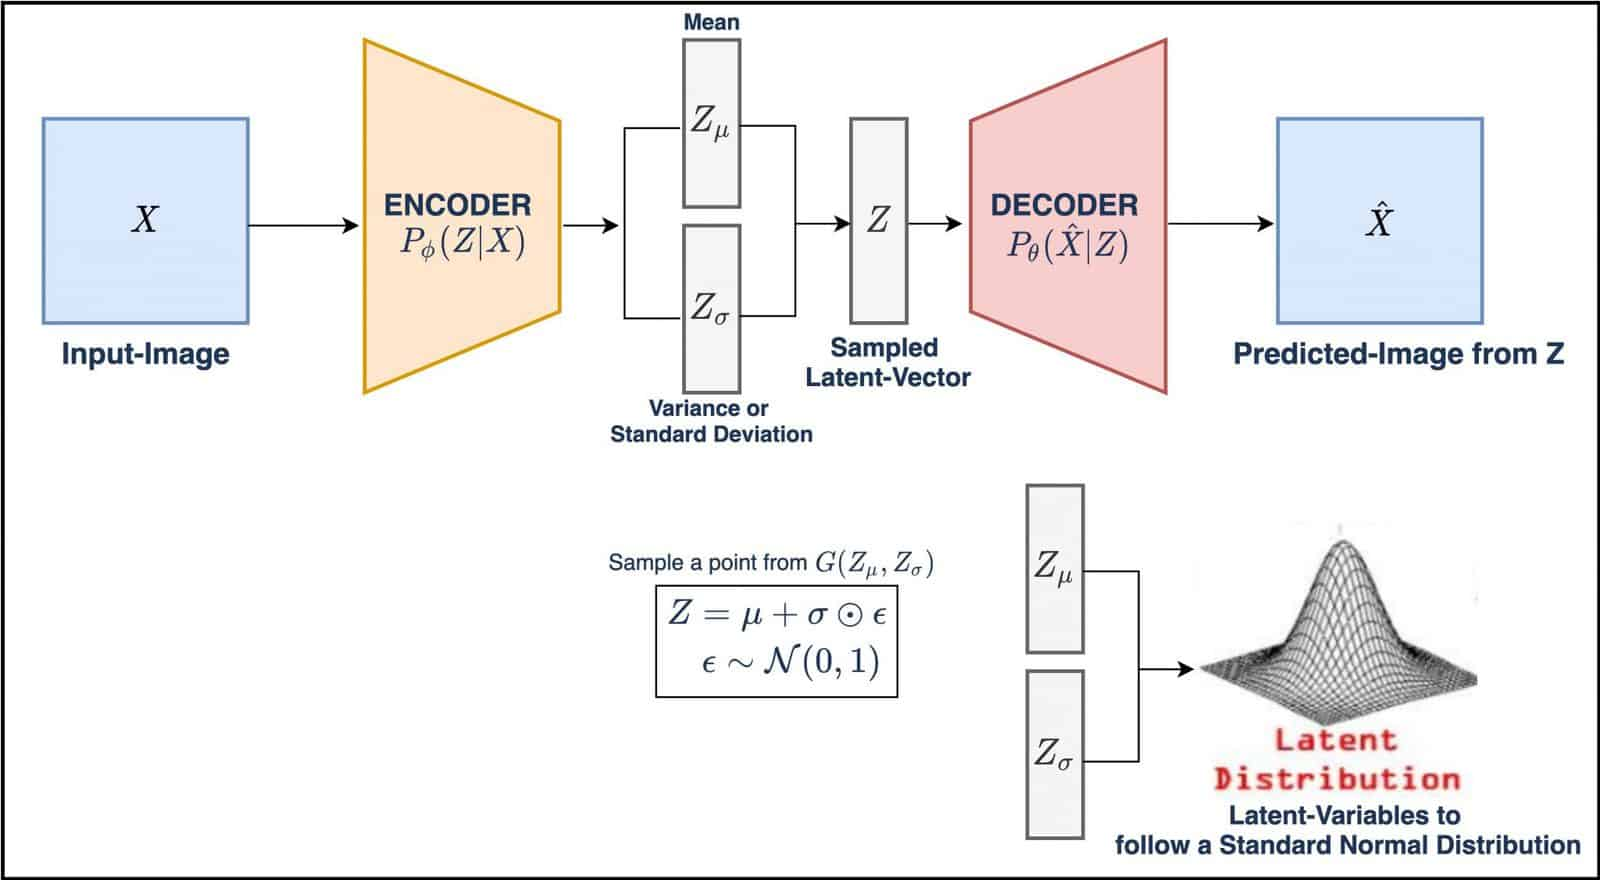
\includegraphics[scale=.125]{vae-diagram.jpg}
        \caption{Source: TODO}
      \end{figure}
      \vspace{-5mm}
      \begin{itemize}
        \item Generative model consisting of probabilisitic encoder and decoder
        \item Encoder \& decoder parametrize probability distributions over latent space and data respectively
      \end{itemize}
      % explain the graphics

    \end{frame}
    \begin{frame}
      \frametitle{Training Variational Autoencoders}
      TODO
     \begin{itemize}
       \item Inspecting Encoder and Decoder
          \item The variational lower bound (ELBO) as on objective and lower bound to the likelihood of data
      % TODO: VAE objective insert and explain
     \end{itemize}
    \end{frame}

    \begin{frame}
      \frametitle{Shortcomings}
      \begin{itemize}
        \item \enquote{low dimensional} latent space $\to$ blurry reconstructions (lack of information in latents)
        \item \enquote{high dimensional} latent space $\to$ low degree of distentanglement and no regularity
        % TODO: Learned distribution in high dimensional space has disperded support -> no regularity
      \end{itemize}
    \end{frame}


    \begin{frame}
      \frametitle{Trying to Fix VAEs}
      \begin{itemize}
        \item change of optimization objective to encourage desired behavior
        \item All about trade-off between reconstruction and disentaglement
        \item Important condition on new objectives: Lower bound to log likelihood of data
        \begin{enumerate}
          \item $\beta$-VAE ($\beta > $ 1): Poor reconstruction (information retained in latent rep. not sufficient)
          \item Factor VAE:
          \item ...
        \end{enumerate}
      \end{itemize}
    \end{frame}


    \section{TC-VAEs}
    \begin{frame}
      \frametitle{Prerequisites}
      \begin{itemize}
        \item $X = (X_{1}, \dots, X_{d})$ random variable (rv) w/ density $p(x)$ and distribution $P^{X}$
        \item $Z = (Z_{1}, \dots, Z_{m})$ rv w/ density $p(z)$ and distribution $P^{Z}$
      \end{itemize}
    \end{frame}

    \begin{frame}
      \frametitle{Shannon Entropy}
      \begin{definition}[Shannon Entropy]
        $H(X) \coloneqq -\mathbb{E}_{P^{X}}[\log p(x)] = -\int_{\R^{d}}p(x) \log p(x) dx$
      \end{definition}
      % Note: def for rv continous, in discrete case, replace Rd by N and dx by counting measure
      % Note: def is equivalent for conditional distributions
      \begin{intuition}
       Measures the randomness of a random variable.
     \end{intuition}
     \begin{example}
       \begin{itemize}
         \item Dirac Measure in a point $\rightarrow H(X) = 0$
               \item Coin Flip $\rightarrow H(X) = 1$
       \end{itemize}
     \end{example}
    \end{frame}


    \begin{frame}
      \frametitle{Mutual Information}
      \begin{definition}[Mutual Information]
        $I(X, Z) \coloneqq H(X) + H(Z) - H(X, Z) = H(X) - H(X \mid Z)$
      \end{definition}
      % Note: def for rv continous, in discrete case, replace Rd by N and dx by counting measure
      \begin{intuition}
        Reduction in uncertainty of one rv given another rv.
        % Or what is left actually. Understand this
      \end{intuition}
    \end{frame}

    \begin{frame}
      \frametitle{Kullback-Leibler Divergence}
      \begin{definition}[Kullback-Leibler Divergence ($D_{KL}$)]
        $I(X, Z) \coloneqq H(X) + H(Z) - H(X, Z) = H(X) - H(X \mid Z)$
      \end{definition}
      % Note: def for rv continous, in discrete case, replace Rd by N and dx by counting measure
      \begin{intuition}
        Reduction in uncertainty of one rv given another rv.
        % Or what is left actually. Understand this
      \end{intuition}
    \end{frame}

    \begin{frame}
      \frametitle{Total Correlation}
      \begin{definition}[Total Correlation (TC)]
        $TC(X) \coloneqq D_{KL}\left[P^{X} \large  \Vert \prod_{i=1}^{d}P^{{X_{i}}}\right] $
      \end{definition}
      \begin{intuition}
        TC measures the amount of information \textit{shared} among the random variables.
        % point out why using the definition
      \end{intuition}
    \end{frame}

    \begin{frame}
      \frametitle{Total Correlation as an objective (1)}
      New objective given by
      \begin{align*}
        \underset{\theta}{\arg \max}TC_{\theta}(Z, X) \coloneqq TC_{\theta}(Z) - TC_{\theta}(Z \mid X).
      \end{align*}
      \begin{intuition}
        Equivalent to minimizing 2nd term $\iff$ given $X$, information shared among components of $Z$ is reduced.
        \newline
        More intuition if viewd in information theoretic framework.
      \end{intuition}
    \end{frame}
    % Why this objective? More insight from information theoretic pov

    \begin{frame}
      \frametitle{Total Correlation as an objective (2)}
      Rewrite TC in terms of MI:
      \begin{align*}
        TC(Z, X) = \left(\sum_{k=1}^{m}I_{\theta}(Z_{k}, X)\right) - I_{\theta}(Z, X)
      \end{align*}

      \begin{intuition}
        \begin{itemize}
          \item Maximizing each terms $I(Z_{k}, X)$ $\to$ promotes single latent variable to \enquote{share} information with $X$
          \item Minimizing $I(Z, X)$ promotes independence of $Z$ conditional on $X$
          % see this by writing I(Z, X) = I(X) - I(X | Z) = I(Z) - I(Z | X) which is minimized if Z is independent condiitonal on X

        \end{itemize}
      \end{intuition}
    \end{frame}

    \begin{frame}
      \frametitle{Total Correlation as an objective (3)}
      \begin{itemize}
        \item Combination of different terms promoting different behavior (VIB, CEB, reconstruction error)
        \item Hyperparameter $\alpha$
        \item Explanation of the single terms - give an intuition
      \end{itemize}
    \end{frame}
    \begin{frame}
      \frametitle{A convex lower bound}
      \textbf{Problem}: Intractable optimization problem. $\to$ need lower bound to maximize.
      Presenting the TC convex lower bound actually used in optimization
    \end{frame}


  \section{Experiments and Results}
    \begin{frame}
      \frametitle{Experiment Design}
      \begin{itemize}
        \item \textbf{Baseline Models}: $\beta$-VAE, Factor VAE
        \item \textbf{Datasets}: 3D shapes dataset and unbalanced 3D shapes dataset, $\dots$
        %% explain U3D shapes dataset
        \item \textbf{Evaluation Methods}:
          \begin{enumerate}
            \item Qualitative: Latent space traversals
            \item Quantitative: DCI, WSEPIN measuring Disentanglement, Completeness and Infromativeness
          \end{enumerate}
      \end{itemize}
    \end{frame}

    \begin{frame}
      \frametitle{Results - Qualitative}
      \begin{itemize}
        \item Traversals through latent space show discovery of 2 OOD generative factors in 3D objects dataset
      \end{itemize}
      \begin{figure}
        \centering
        \includegraphics[scale=0.2]{latent_traversals_TC.png}
        \captionsetup{justification=centering}
        \caption*{\tiny{Source: original paper}}
        % understand how this image is generated, how do traversals work?

      \end{figure}
    \end{frame}

    \begin{frame}
      \frametitle{Results - Quantitative}
      \begin{itemize}
        \item Outperforming baseline models on balanced dataset in terms of presented evaluation metrics

        \item Performance on unbalanced datasets falls short of performance of baseline models
      \end{itemize}
    \end{frame}

  \section{Discussion and Conclusion}
    \begin{frame}
      \frametitle{Discussion and Conclusion}
      \begin{itemize}
        \item Inspiration from Multiview representation learning (OOD generative factors correspond to missing views)
        \item Uncovering OOD generative factors $\equiv$ inferring missing views
        \item Experimental validation that TC-VAE is capable of uncovering OOD generative factors
        \item missing view also problematic for downstream tasks. underrepresented views may be seen as outliers
        \item main shortcoming: Terms appearing as part of the bound do promote conflicting behavior during minization
        \item unbalanced generative factors in dataset $\implies$ disentanglement deteriorates.
      \end{itemize}
    \end{frame}


    \begin{frame}
      \frametitle{Criticism}
      \begin{enumerate}
              \item The concept of disentanglement is not clearly defined. Sometimes its equivalent to independence, sometimes not.
      \end{enumerate}
    \end{frame}


    \begin{frame}
      \frametitle{Opinion}
      \begin{itemize}
        \item Lack of formalization of the concept of disentaglement
        \item Not clear which definitions of TC they are using. Although they are citing the MVRL paper quite often, the deifnition of TC does not match



      \end{itemize}

    \end{frame}


    \begin{frame}
      \frametitle{Literature}
      Book Elements of information theory
    \end{frame}


   \end{document}
